\subsection{All to finish application}
    We can extend the previous application to an all-to-finish operator. This operator can for instance represent parallel work: a task that requires a lot of computation and can be done in separate pieces by separate workers. \cite{dq-tut} \\
    The outcome diagram is the one we presented in \cref{fig:op}. It can be represented textually by:
    \begin{minted}{text}
        ... = a:atf(worker_1, worker_2);
    \end{minted}

        \subsubsection{Introducing a slower component}
            Like we did for the FTF operator, let's introduce a slower worker into the system. We introduce a slight delay to show how even a few milliseconds can be noticeable right away by a keen eye (or by triggers, which avoids having to look constantly at the graphs). Worker\_2 is 2ms slower.
 
            The difference in the worker's $\Delta$Q can be noticed with $\Delta \text{Q}_{w2} > \Delta \text{Q}_{w1}$ on the right in \cref{fig:slower_atf}. The difference can then be observed in the all-to-finish plot on the left in \cref{fig:slower_atf}, where the operator's $\Delta$Qs confidence bounds (both observed and calculated) can be overlaid on top of worker\_2 $\Delta$Q. This shows once again that the $\Delta$QSD algebraic foundation is sound. Moreover, the oscilloscope can be useful in detecting slower components in a system.

            \begin{figure}[H]
                \begin{center}
                    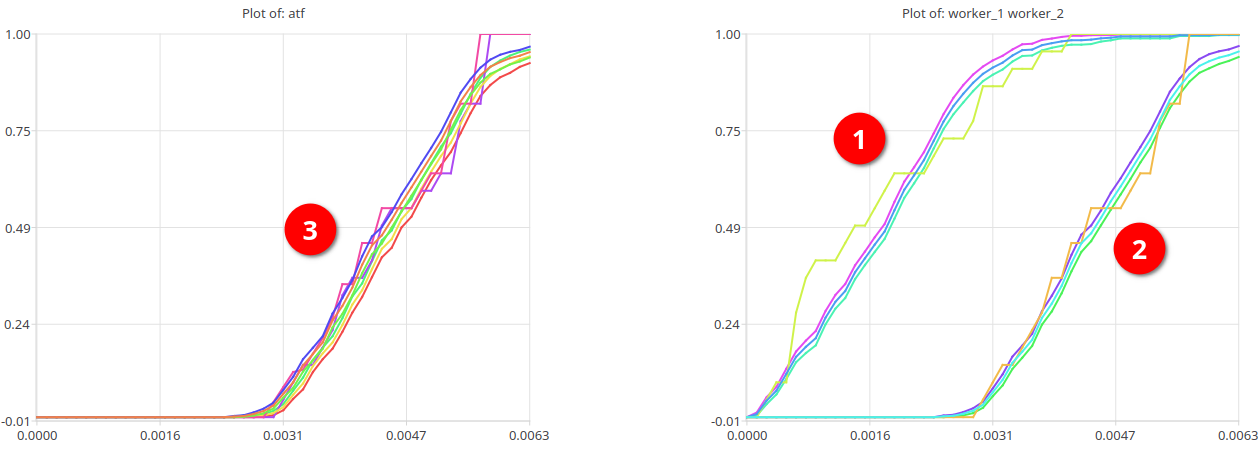
\includegraphics[scale = 0.5]{img/overload_2/w1w2atfa.png}
                \end{center}
                \caption{\textbf{Left}: ATF plot with observed and calculated $\Delta$Q confidence bounds overlapping. \textbf{Right}: Worker's plots, worker\_2 (2) is slower than worker\_1 (1).}
                \label{fig:slower_atf}
            \end{figure}

    These plots show the usefulness of $\Delta$QSD, the system can be decomposed to understand which part of the system is showing hazards thanks to the notion of outcome diagrams. Furthermore, the causal relationships can be observed to determine the behaviour of a part down to the single component.
